\documentclass[a4paper,11pt]{article}
\usepackage[portuguese]{babel}
\usepackage{graphicx}
\usepackage{amsmath}
\usepackage{enumitem}
\usepackage{fancyvrb}

\usepackage[twoside,verbose,body={16cm,24cm},
left=25mm,top=20mm]{geometry}

\title{Algoritmos e Complexidade\\ Ficha 2: Resolução}

\author{Eduardo Freitas Fernandes}
\date{2025}

\begin{document}
	
	\maketitle
	
	\section{Contagem}
	
	\textbf{Exercício 1}\\
	
	\noindent \textbf{Função \texttt{bubbleSort()}}:\\
	
	\noindent \textbf{Comparações entre elementos do array}:
	O número de comparações entre elementos do array é igual em todos os casos, isto é, o conteúdo do array não altera a execução da função, logo o melhor e pior caso terão o mesmo custo.\\
	\[
		T_{bubbleSort}(N) = \sum_{i=1}^{N-1} \sum_{j=0}^{i-1} 1 = \sum_{i=1}^{N-1} i = \frac{(N-1) \times N}{2} = \Theta(N^2)
	\]
	
	\noindent \textbf{Trocas Efetuadas}:
	\begin{itemize}
		\item \textbf{Melhor caso}: array ordenado por ordem crescente (condição do \texttt{if statement} é sempre falsa)
		\item \textbf{Pior caso}: array ordenado por ordem decrescente (condição do \texttt{if statement} é sempre verdadeira)
	\end{itemize}
	
	\noindent \textbf{Função \texttt{iSort()}}:\\
	
	\noindent \textbf{Comparações entre elementos do array}:
	\begin{itemize}
		\item \textbf{Melhor caso}: array ordenado por ordem crescente (apenas uma comparação no loop interno, de cada iteração do loop externo)
		\[ T_{iSort}(N) = \sum_{i=1}^{N-1} 1 = N-1 = \Omega(N) \]
		\item \textbf{Pior caso}: array ordenado por ordem decrescente
		\[ T_{iSort}(N) = \sum_{i=1}^{N-1} \sum_{j=1}^{i} 1 = \sum_{i=1}^{N-1} i = \frac{N^2 - N}{2} = O(N^2) \]
	\end{itemize}
	
	\noindent Para as trocas de elementos, o melhor e pior caso são os mesmos, dado que o \texttt{swap} depende da condição de paragem do \texttt{for loop}.\\
	
	\newpage
	
	\noindent \textbf{Exercício 2}\\
	
	\noindent Seja N o número de bits necessários para representar \texttt{x}, teremos a seguinte gama de valores:
	\begin{itemize}
		\item $ 2^{N-1} $, que corresponde a todos os bits excepto o mais significativo serem 0 (melhor caso)
		\item $ \sum_{k=0}^{N-1} 2^k = 2^N - 1 $, no caso dos bits serem todos 1 (pior caso)
	\end{itemize}
	
	\noindent \textbf{Função \texttt{mult1()}}:\\
	
	\noindent O número de somas e subtrações é igual, logo não é necessário especificar cada um. O número de operações primitivas (\texttt{+ -}) no \textbf{pior caso} será:
	
	\[ T_{mult1}(N) = 2^N - 1 = \Theta(2^N) \]
	
	\noindent \textbf{Função \texttt{mult2()}}:\\
	
	\noindent No pior caso, todos os bits estão a 1, logo a condição avaliada no \texttt{if statement} será sempre verdadeira, então a operação primitiva \texttt{+} será executada tantas vezes quanto as operações \texttt{\% / *}. Podemos concluir que a complexidade é \textbf{linear}, em função do número de bits, pois a cada iteração um dos bits de \texttt{x} passa a 0 e é efetuada uma adição.\\
	
	
	\noindent \textbf{Exercício 3}
	
	\[
		T(N) = \sum_{i=0}^{N-1} \sum_{j=i}^{N-1} \sum_{k=i}^{j} 1 = \sum_{i=0}^{N-1} \sum_{j=i}^{N-1} j-i+1 = \sum_{i=0}^{N-1} \sum_{j=i}^{N-1} j	
	\]
	\[
		= \sum_{i=0}^{N-1} \frac{(N-i) \times (N-1+i)}{2} = \sum_{i=0}^{N-1} \frac{N^2 + ...}{2} = \frac{N^3}{3} + ... = \Theta(N^3)
	\]
	
	\noindent \textbf{Nota}: na resolução deste somatório decidi remover a expressão $ -i + 1 $ devido ao facto de ser uma constante no segundo somatório, então teria pouco impacto no resultado final da complexidade e iria dificultar os cálculos.
	
\begin{Verbatim}[tabsize=4]
int maxSoma(int v[], int N) {
	int max, i, t;
	int c[N];
	c[0] = v[0];
	max = c[0];
	for (i = 1; i < N; i++) {
		t = c[i - 1] + v[i];
				
		if (t > c[i - 1]) c[i] = t;
		else c[i] = v[i];
				
		if (c[i] > max) max = c[i];
	}
	return max;
}
	\end{Verbatim}
	\[
	T_{maxSoma}(N) = 1 + \sum_{i=1}^{N-1} 2 = 1 + 2 \times (N-1) = \Theta(N)
	\]
	
	
	\noindent \textbf{Exercício 4}\\
	
	\noindent Comparações entre elementos do array:
	
	\begin{itemize}
		\item \textbf{Melhor Caso}: array estritamente decrescente
		\item \textbf{Pior Caso}: array estritamente crescente
	\end{itemize}
	\[
		T_{maxcresc}(N) = \sum_{i=0}^{N-1} \sum_{j=1}^{N-1} 1 = \sum_{i=0}^{N-1} N - 1 = N \times (N-1) = O(N^2)
	\]
	
	\noindent Ao realizar a optimização \texttt{i += m}, serão efetuadas apenas \texttt{N} comparações, pois \texttt{m} terá o valor \texttt{N}, pondo fim ao ciclo. Isto acontece porque o array está ordenado por ordem crescente, então \texttt{m} será o comprimento do maior segmento crescente, que corresponde a \texttt{N}.
	
	
	\section{Definições Recursivas}
	
	\noindent \textbf{Exercício 1}\\
	
	\noindent a)
	
	\begin{figure}[h]
		\centering
		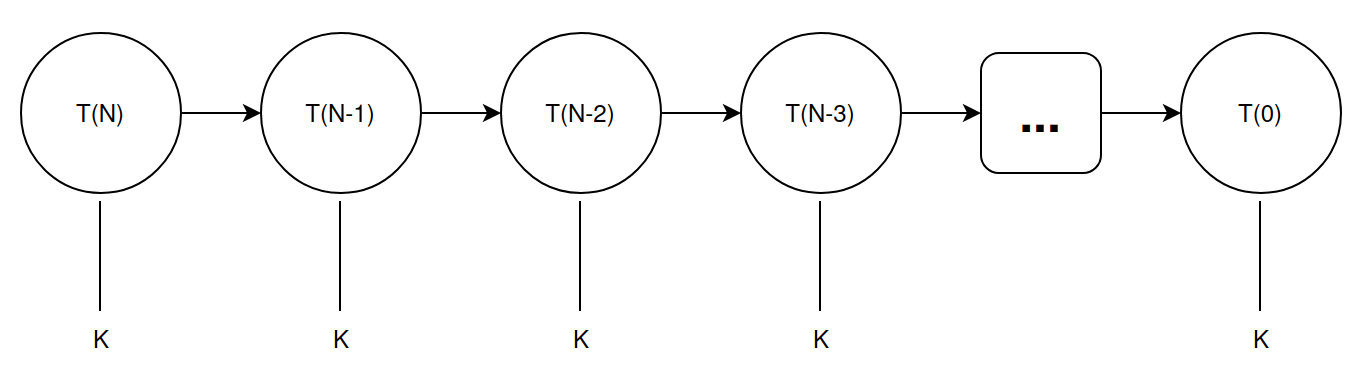
\includegraphics[width=0.8\textwidth]{imgs/2_1-a.png}
	\end{figure}
	\[
		T(N) = \sum_{i=0}^{N} K = (N + 1) \times K = \Theta(N)
	\]
	
	\noindent b)
	
	\begin{figure}[h]
		\centering
		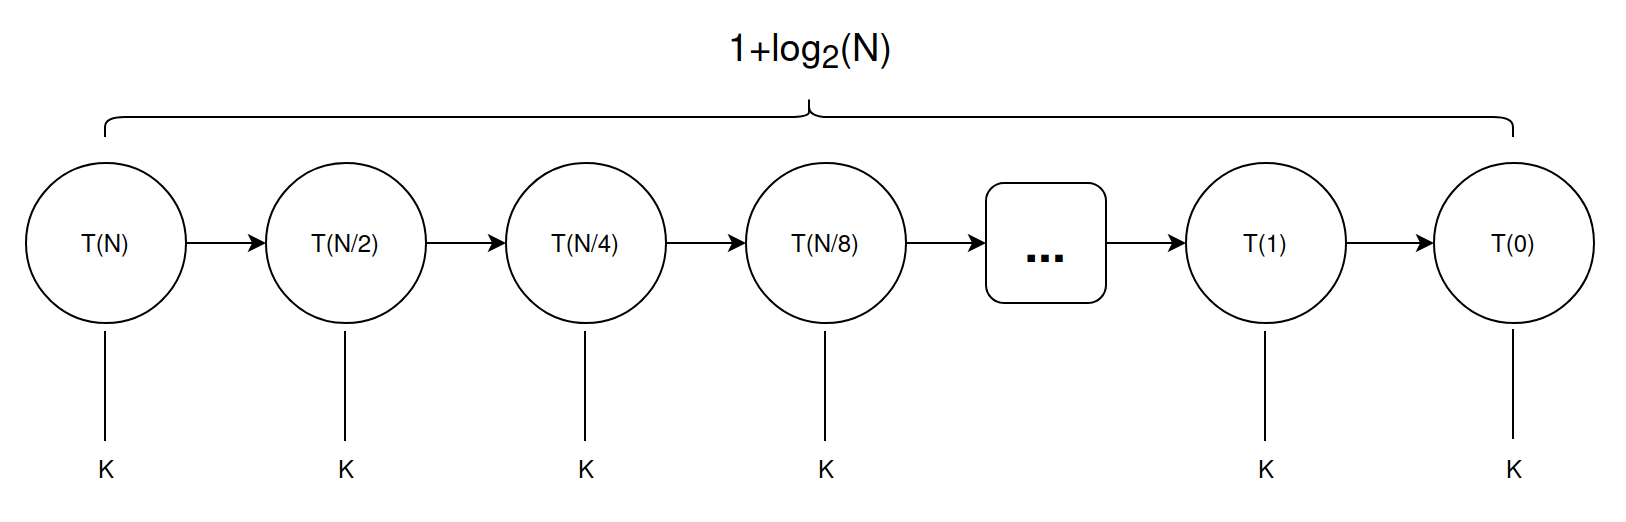
\includegraphics[width=0.8\textwidth]{imgs/2_1-b.png}
	\end{figure}
	\[
		T(N) = \sum_{i=0}^{1 + \log_2(N)} K = (2 + \log_2(N)) \times K = \Theta(\log_2(N))
	\]
	
	\newpage
	
	\noindent c)
	
	\begin{figure}[h]
		\centering
		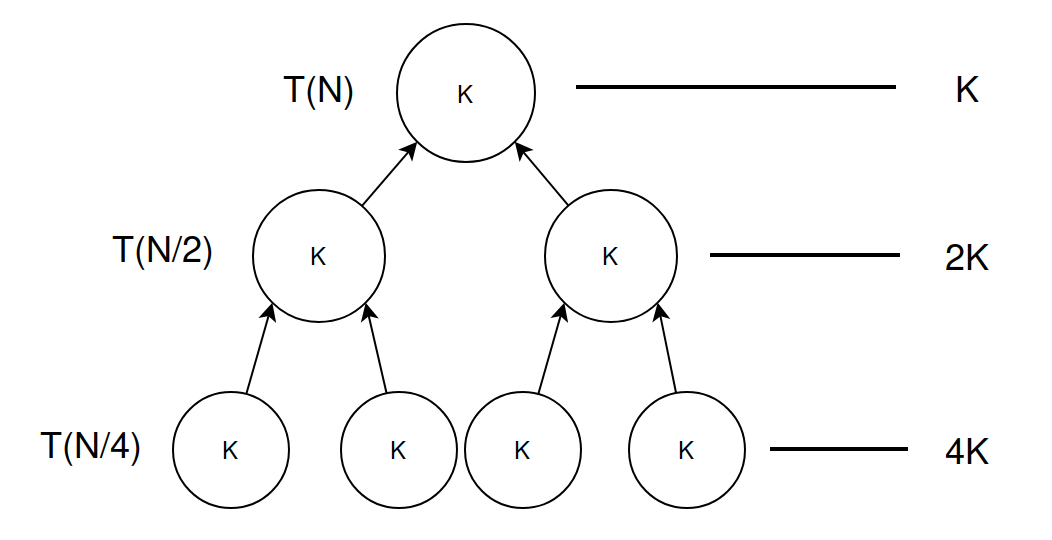
\includegraphics[width=0.6\textwidth]{imgs/2_1-c.png}
	\end{figure}
	\[
		T(N) = \sum_{i=0}^{1 + \log_2(N)} 2^i \times K = K \times (2^{\log_2(N) + 2} - 1) = K \times (4 \times N - 1) = \Theta(N)
	\]
	
	\noindent d)
	
	\begin{figure}[h]
		\centering
		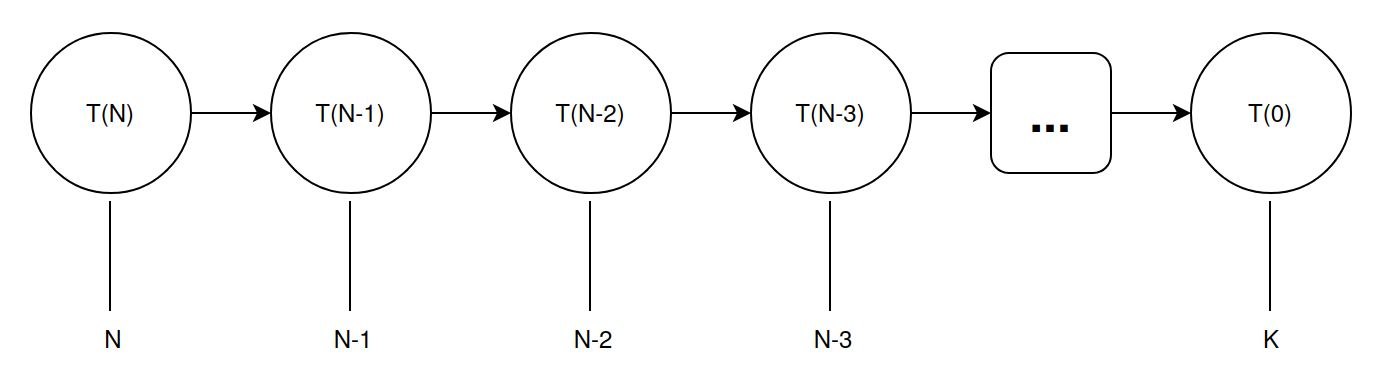
\includegraphics[width=0.8\textwidth]{imgs/2_1-d.png}
	\end{figure}
	\[
		T(N) = K + \sum_{i=1}^{N} i = K + \frac{N \times (N + 1)}{2} = \Theta(N^2)
	\]
	
	\noindent e)
	
	\begin{figure}[h]
		\centering
		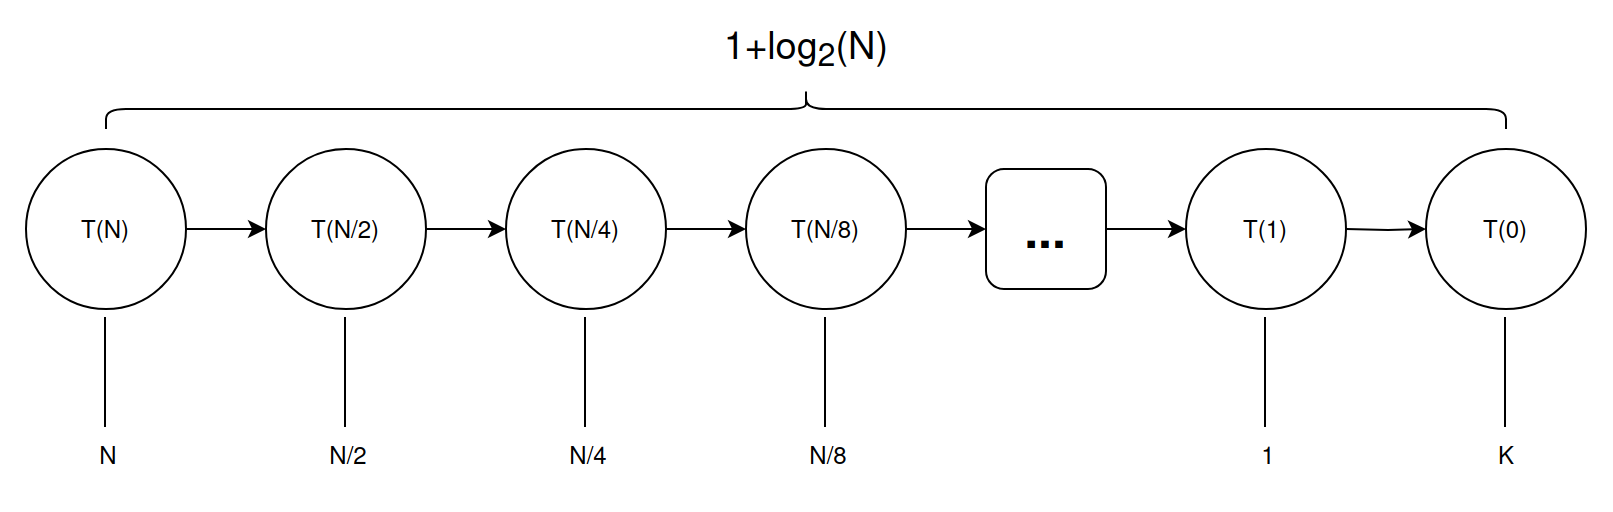
\includegraphics[width=0.8\textwidth]{imgs/2_1-e.png}
	\end{figure}
	\[
		T(N) = K + \sum_{i=1}^{1 + \log_2(N)} \frac{N}{2^i} = K + 2^{\log_2(N) + 1} - 1 = K + 2 \times N - 1 = \Theta(N)
	\]
	
	\newpage
	
	\noindent f)
	
	\begin{figure}[h]
		\centering
		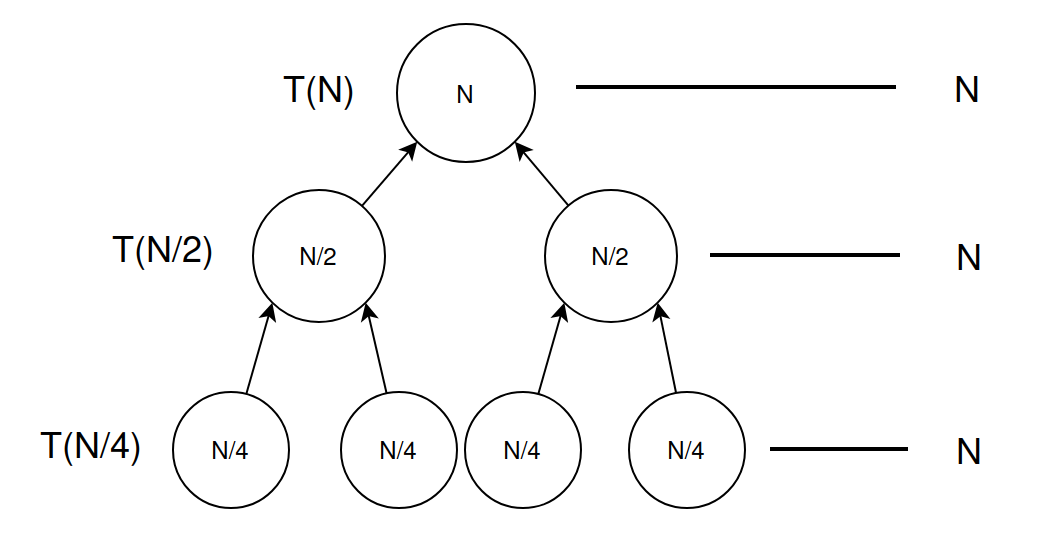
\includegraphics[width=0.6\textwidth]{imgs/2_1-f.png}
	\end{figure}
	\[
		T(N) = K + \sum_{i=1}^{1 + \log_2(N)} N = K + N \times (1 + \log_2(N)) = \Theta(N \times \log_2(N))
	\]
	
	\noindent \textbf{Exercício 2}
	
	\[
		T(N) =
		\begin{cases}
			0 & N \leq 0 \\
			1 + N - 1 + T(N - 1) & N > 0
		\end{cases}
		\quad = \quad
		\begin{cases}
			0 & N \leq 0 \\
			N + T(N - 1) & N > 0
		\end{cases}
	\]
	\[
		= \sum_{i=1}^{N} i = \frac{N \times (N + 1)}{2} = \Theta(N^2)
	\]
	
	
	\noindent \textbf{Exercício 3}
	
	\[
		T(N) = 
		\begin{cases}
			0 & N \leq 0 \\
			1 + 2 \times T(N - 1) & N > 0
		\end{cases}
	\]
	
	\begin{figure}[h]
		\centering
		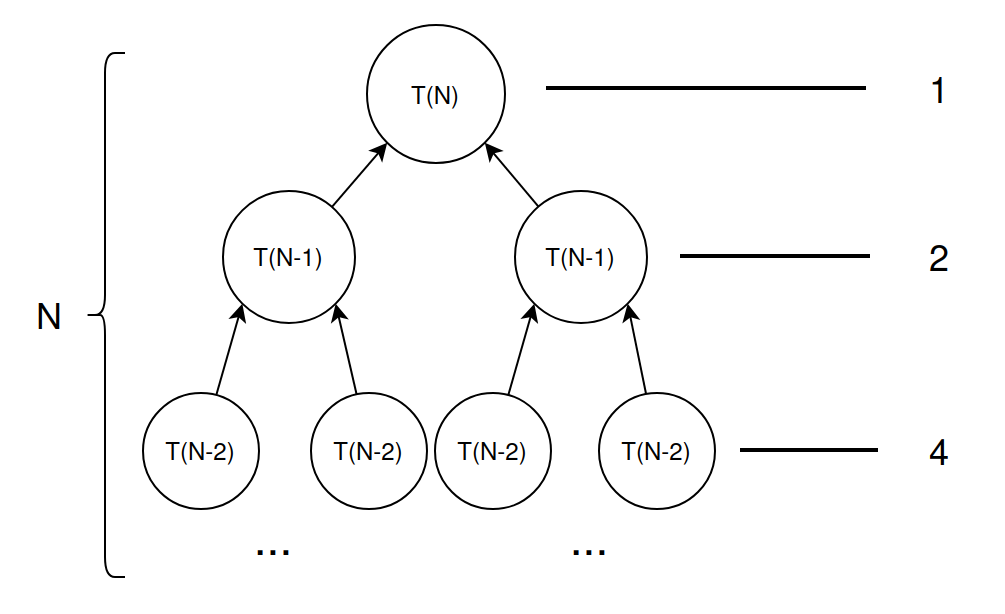
\includegraphics[width=0.7\textwidth]{imgs/2_3.png}
	\end{figure}
	
	\[
		T(N) = \sum_{i=0}^{N-1} 2^i = 2^N - 1 = \Theta(2^N)
	\]
	
	\newpage
	
	\noindent \textbf{Exercício 4}
	
	\[
		T(N) = 
		\begin{cases}
			1 & N \leq 1 \\
			T_{mergeH}(N) + 2 \times T(N / 2) & N > 1
		\end{cases}
		=
		\begin{cases}
			1 & N \geq 1 \\
			2 \times N + 2 \times T(N/2) & N > 1
		\end{cases}
	\]
	
	\[
		= \sum_{i=1}^{1 + \log_2(N)} 2 \times N = 2 \times N \times (1 + \log_2(N)) = \Theta(N \times \log_2(N))
	\]
	
	\noindent \textbf{Exercício 5}\\
	
	\noindent \textbf{Árvores Equilibradas}
	
	\[
		T(N) = 
		\begin{cases}
			0 & N \leq 0 \\
			1 + 2 \times T(\frac{N-1}{2}) & N > 0
		\end{cases}
		=
		\begin{cases}
			0 & N \leq 0 \\
			1 + 2 \times T(N/2) & N > 0
		\end{cases}
	\]
	\[
		= \sum_{i=0}^{1 + \log_2(N)} 2^i = 4 \times N - 1 = \Theta(N)
	\]
	
	\noindent \textbf{Árvores "Lista"}
	
	\[
	T(N) = 
	\begin{cases}
		0 & N \leq 0 \\
		1 + T(N - 1) & N > 0
	\end{cases}
	\quad = \quad \sum_{i=1}^{N} 1 = N = \Theta(N)
	\]
	
	
	
	\section{Análise de Caso Médio}
	
	\noindent \textbf{Exercício 1}
	
	\noindent \textbf{Exercício 2}
	
	\noindent \textbf{Exercício 3}
	
	\noindent \textbf{Exercício 4}
	
	\noindent \textbf{Exercício 5}
	
	\noindent \textbf{Exercício 6}
	
	
	\section{Análise Amortizada}
	
	\noindent \textbf{Exercício 1}
	
	\noindent \textbf{Exercício 2}
	
	\noindent \textbf{Exercício 3}
	
	
\end{document}